%-------------------------------------------------------------------------------
% PRÉAMBULE - CONFIGURATION DU DOCUMENT
%-------------------------------------------------------------------------------
\documentclass[11pt,a4paper]{report}

%----- Packages essentiels -----------------------------------------------------
\usepackage[utf8]{inputenc}
\usepackage[T1]{fontenc}
\usepackage[french]{babel}
\usepackage{geometry}
\geometry{top=2.5cm, bottom=2.5cm, left=2.5cm, right=2.5cm}
\usepackage{graphicx}
\usepackage{float}
\usepackage{caption}
\usepackage{subcaption}
\usepackage{amsmath, amssymb}
\usepackage{booktabs}
\usepackage{array}
\usepackage{colortbl}
\usepackage{xcolor}
\usepackage{hyperref}
\hypersetup{
    colorlinks=true,
    linkcolor=blue,
    urlcolor=blue,
    citecolor=black,
    bookmarksdepth=3
}
\usepackage{fancyhdr}
\setlength{\headheight}{14pt}
\usepackage{setspace}
\setstretch{1.15}
\usepackage{listings}
\usepackage{enumitem}
\usepackage{titlesec}
\usepackage{longtable}
\usepackage{multirow}
\usepackage{tikz}
\usepackage{url}
\usepackage{eurosym}
\usetikzlibrary{positioning,shapes,arrows,fit,shapes.geometric}

%----- Définition de \ieme pour l'ordinal français ----------------------------
\renewcommand{\ieme}{\textsuperscript{ème}}

%----- Mise en forme des titres -----------------------------------------------
\titleformat{\section}{\normalfont\fontsize{14}{16}\bfseries}{\thesection}{1em}{}
\titleformat{\subsection}{\normalfont\fontsize{12}{14}\bfseries}{\thesubsection}{1em}{}
\titleformat{\subsubsection}{\normalfont\fontsize{11}{13}\bfseries}{\thesubsubsection}{1em}{}

%----- Espacement des titres (réduction des blancs) ---------------------------
\titlespacing*{\chapter}{0pt}{-30pt}{15pt}
\titlespacing*{\section}{0pt}{8pt}{4pt}
\titlespacing*{\subsection}{0pt}{6pt}{3pt}
\titlespacing*{\subsubsection}{0pt}{4pt}{2pt}

%----- Listes compactes -------------------------------------------------------
\setlist{
  topsep=2pt,
  itemsep=1pt,
  parsep=0pt,
  partopsep=0pt
}

%----- Espaces autour des figures et tableaux ---------------------------------
\setlength{\textfloatsep}{10pt}
\setlength{\floatsep}{8pt}
\setlength{\intextsep}{8pt}

%----- Espacement inter-paragraphes -------------------------------------------
\setlength{\parskip}{3pt}

%----- Tableaux plus compacts -------------------------------------------------
\renewcommand{\arraystretch}{0.9}

%----- Configuration des listes de code ---------------------------------------
\lstset{
    language=Python,
    basicstyle=\ttfamily\footnotesize,
    keywordstyle=\color{blue},
    commentstyle=\color{green!50!black},
    stringstyle=\color{red},
    numbers=left,
    numberstyle=\tiny\color{gray},
    frame=single,
    breaklines=true,
    captionpos=b,
    extendedchars=true,
    literate=
      {é}{{\'e}}1
      {è}{{\`e}}1
      {à}{{\`a}}1
      {ù}{{\`u}}1
      {ç}{{\c{c}}}1
      {œ}{{\oe}}1
      {É}{{\'E}}1
      {È}{{\`E}}1
      {À}{{\`A}}1
      {Ç}{{\c{C}}}1
}

%----- Configuration JavaScript pour listings ---------------------------------
\lstdefinelanguage{JavaScript}{
    keywords={typeof, new, true, false, catch, function, return, null, catch, switch, var, if, in, while, do, else, case, break, const, let, await, async, fetch},
    keywordstyle=\color{blue}\bfseries,
    ndkeywords={class, export, boolean, throw, implements, import, this},
    ndkeywordstyle=\color{darkgray}\bfseries,
    identifierstyle=\color{black},
    sensitive=false,
    comment=[l]{//},
    morecomment=[s]{/*}{*/},
    commentstyle=\color{green!50!black}\ttfamily,
    stringstyle=\color{red}\ttfamily,
    morestring=[b]',
    morestring=[b]"
}

%----- En-têtes et pieds de page ----------------------------------------------
\pagestyle{fancy}
\fancyhf{}
\fancyhead[L]{\small\textit{Système d'Orientation Clinique Multi-Agents}}
\fancyhead[R]{\small\textit{\thepage}}
\fancyfoot[C]{}

%----- Définition de commandes personnalisées ---------------------------------
\newcommand{\HRule}{\rule{\linewidth}{0.5mm}}

%----- Couleurs pour les tableaux ---------------------------------------------
\definecolor{gray95}{gray}{0.95}
\definecolor{gray90}{gray}{0.90}
\definecolor{lightblue}{RGB}{173,216,230}
\definecolor{bleuPro}{RGB}{0,112,192}
\newcolumntype{P}[1]{>{\centering\arraybackslash}p{#1}}

%-------------------------------------------------------------------------------
% DEBUT DU DOCUMENT
%-------------------------------------------------------------------------------
\begin{document}

% Forcer la numérotation arabe
\pagenumbering{arabic}
\setcounter{page}{1}

% ================= PAGE DE GARDE =================
\begin{titlepage}
    \centering
    \vspace*{0.5cm}

    
\includegraphics[width=0.45\textwidth]{logo_emsi.png}

    \vspace{0.6cm}
    {\color{bleuPro}\rule{0.9\textwidth}{1.5pt}}

    \vspace{0.6cm}
    {\Large \textbf{École Marocaine des Sciences de l'Ingénieur}}\\
    {\large EMSI Casablanca — IA \& Big Data}

    \vspace{0.4cm}
    {\color{bleuPro}\rule{0.9\textwidth}{0.7pt}}

    \vspace{1cm}

    {\large \textbf{Rapport de Projet de Fin d'Année}}

    \vspace{0.2cm}
    {\large 4\ieme{} Année Ingénierie (4IAD G2)}\\

    \vspace{1cm}

    {\Huge \textbf{Système Multi-Agents d'Orientation Clinique Préliminaire avec LangGraph et Protocole MCP}}\\
    \vspace{0.5cm}
    {\large \textit{Intégration d'un workflow d'orientation conversationnel dynamique, RAG médical avec Tavily et boucle de validation Physician-in-the-Loop}}

    \vspace{1.5cm}

    \begin{minipage}{0.9\textwidth}
        \centering
        {\large \textbf{Réalisé par :}}\\
        {\large \textbf{AYOGNIDE Riyadh Akorede Atanda}}\\
        \vspace{0.8cm}
        {\large \textbf{Encadré par :}}\\
        {\large \textbf{M. Khalid EL AMRAOUI}}\\
        \vspace{0.8cm}
        {\large \textbf{Dépôt GitHub :}}\\
        {\small \url{https://github.com/riyadh03/IA_medical_assistant}}
    \end{minipage}

    \vfill

    {\large Année universitaire 2025-2026}
\end{titlepage}

%----- DÉDICACES --------------------------------------------------------------
\newpage
\section*{Dédicaces}
\addcontentsline{toc}{section}{Dédicaces}
\vspace*{2cm}
\begin{center}
    \textit{À ma famille, pour leur soutien inconditionnel et leur amour constant tout au long de mon parcours universitaire.}\\
    \vspace{1cm}
    \textit{À mes enseignants de l'EMSI, qui m'ont fourni les bases et m'ont encouragé à explorer le domaine de l'intelligence artificielle agentique.}\\
    \vspace{1cm}
    \textit{À mes camarades de promotion, avec qui j'ai partagé des moments d'effort et d'entraide.}
\end{center}

%----- REMERCIEMENTS ----------------------------------------------------------
\newpage
\section*{Remerciements}
\addcontentsline{toc}{section}{Remerciements}

Je tiens à exprimer ma profonde gratitude et mes sincères remerciements à toutes les personnes qui ont contribué au succès de ce travail académique.

Mes remerciements s'adressent tout particulièrement à mon encadrant, \textbf{Monsieur Khalid EL AMRAOUI}, pour sa patience, ses précieux conseils scientifiques, et ses orientations techniques rigoureuses. Son expertise dans le domaine de l'intelligence artificielle et de l'ingénierie logicielle a été un guide indispensable tout au long de la conception et du développement de ce projet.

Je remercie également l'ensemble du corps professoral de l'\textbf{École Marocaine des Sciences de l'Ingénieur (EMSI)} pour la qualité de l'enseignement reçu et les ressources mises à notre disposition. 

Enfin, j'exprime ma gratitude aux membres du jury qui ont accepté d'évaluer ce travail de fin d'année.

\newpage

%----- RESUME (en francais) ----------------------------------------------------------
\section*{Résumé}
\addcontentsline{toc}{section}{Résumé}

Ce projet présente la conception et le développement d'un système intelligent multi-agents dédié à l'orientation clinique préliminaire, orchestré par la bibliothèque \textbf{LangGraph} et exposé sous forme d'architecture REST avec \textbf{FastAPI} et \textbf{Next.js}. Le système vise à automatiser un entretien d'orientation médicale en 5 questions adaptées de manière 100\% dynamique par un LLM en fonction du profil et de la plainte initiale du patient. 

Afin de garantir la rigueur médicale et la sécurité, le système intègre une architecture de recherche dynamique (RAG) connectée au protocole \textbf{Model Context Protocol (MCP)} via l'outil de recherche externe \textbf{Tavily API}, permettant de récupérer des sources cliniques réelles. Un second outil local de sécurité (\textbf{Red Flag Checker}) vérifie en continu la présence d'indicateurs de gravité. En phase finale de l'orientation, un mécanisme \textbf{Human-in-the-Loop} (HITL) suspend l'exécution du graphe pour soumettre le cas à la validation d'un médecin traitant. 

Le système complet est conteneurisé avec \textbf{Docker Compose}, assure une persistance robuste dans une base de données \textbf{SQLite}, et intègre un bouton d'export de rapport final au format PDF généré via une bibliothèque native `jsPDF` côté client, exempte de dépendances externes lourdes.

\vspace{0.5cm}
\textbf{Mots-clés :} LangGraph, FastAPI, Next.js, Model Context Protocol, Multi-Agents, Human-in-the-Loop, RAG Médical, SQLite, Docker Compose, jsPDF.

\newpage

%----- ABSTRACT (en anglais) ----------------------------------------------------------
\section*{Abstract}
\addcontentsline{toc}{section}{Abstract}

This project presents the design and implementation of a multi-agent clinical orientation system orchestrated by \textbf{LangGraph} and exposed through a REST API using \textbf{FastAPI} and a \textbf{Next.js} frontend. The system automates a preliminary clinical intake interview consisting of exactly 5 follow-up questions generated dynamically by an LLM based on the patient's demographics and chief complaint.

To ensure clinical accuracy and safety, the system integrates a dynamic retrieval-augmented generation (RAG) architecture using the \textbf{Model Context Protocol (MCP)} with the \textbf{Tavily Search API} to fetch real-time clinical sources. A local security tool (\textbf{Red Flag Checker}) monitors the patient's symptoms for high-risk flags. Upon completing the interview, a \textbf{Human-in-the-Loop} (HITL) mechanism suspends graph execution, awaiting review and confirmation from a licensed physician.

The complete system is containerized with \textbf{Docker Compose}, features persistent storage via \textbf{SQLite}, and provides client-side PDF generation using native `jsPDF`, removing external rendering dependencies.

\vspace{0.5cm}
\textbf{Keywords:} LangGraph, FastAPI, Next.js, Model Context Protocol, Multi-Agent System, Human-in-the-Loop, Medical RAG, SQLite, Docker Compose, jsPDF.

%----- TABLE DES MATIÈRES -----------------------------------------------------
\newpage
\tableofcontents
\newpage

%----- INTRODUCTION GÉNÉRALE --------------------------------------------------
\newpage
\section*{Introduction Générale}
\addcontentsline{toc}{section}{Introduction Générale}

L'avancement technologique des grands modèles de langage (LLM) a permis de dépasser le cadre des agents conversationnels simples à une seule étape pour se diriger vers des architectures multi-agents complexes et collaboratives. Dans les domaines sensibles tels que la santé, ces systèmes offrent d'immenses opportunités pour structurer et optimiser le parcours de soins, en assistant les professionnels dans la pré-analyse des cas patients.

Cependant, l'utilisation de l'intelligence artificielle en milieu médical nécessite d'encadrer strictement les sorties générées afin d'éviter les hallucinations cliniques et les diagnostics erronés. Pour résoudre cette problématique, deux axes de conception majeurs doivent être combinés : d'une part, l'apport de connaissances médicales externes dynamiques via un pipeline RAG (Retrieval-Augmented Generation), et d'autre part, le contrôle systématique par un expert humain, matérialisé par un mécanisme d'interruption "Human-in-the-Loop".

C'est dans ce contexte que s'inscrit le projet de fin d'année présenté dans ce document. Nous avons développé une plateforme d'orientation clinique préliminaire académique. Le système automatise un interrogatoire personnalisé en 5 questions, interroge un serveur MCP pour évaluer les drapeaux rouges et chercher des guidelines de référence, puis interrompt son exécution pour permettre au médecin de valider le dossier avant la génération du rapport final.

Ce rapport s'articule autour de 9 chapitres techniques. Nous aborderons d'abord les objectifs du projet, l'analyse des exigences et l'architecture multi-agents. Nous détaillerons ensuite l'intégration du protocole MCP, la persistance avec SQLite, l'API FastAPI, l'interface Next.js, et la validation par des scénarios cliniques réels, pour conclure sur les limites éthiques et les perspectives d'évolution.

%===============================================================================
% CHAPITRES
%===============================================================================

\chapter{Contexte et Objectifs}
\section{Contexte Technique}
La conception traditionnelle d'applications basées sur les LLM repose souvent sur des modèles simples de type "Prompt-Response". Bien que puissants pour des tâches génériques, ces modèles montrent des limites claires lorsqu'il s'agit de gérer des processus multi-étapes ou des décisions conditionnelles complexes. 
L'orchestration de graphes d'agents (via des bibliothèques comme LangGraph) permet de structurer les interactions sous forme de machines à états cycliques. Chaque agent (nœud) exécute une tâche spécifique (diagnostic, rédaction, contrôle) et transmet son résultat au superviseur qui oriente le flux.

\section{Problématique}
Le principal défi des agents conversationnels médicaux réside dans la précision et la sécurité. Comment modéliser un système autonome capable de poser des questions pertinentes à un patient tout en assurant qu'aucune recommandation médicale ne soit émise sans la relecture et la validation d'un médecin ?

\section{Objectifs du Projet}
Pour répondre à cette problématique, les objectifs suivants ont été fixés :
\begin{itemize}
    \item \textbf{Modélisation de Graphes Cycles} : Utiliser LangGraph pour concevoir un workflow réversible et interruptible.
    \item \textbf{Interrogatoire Clinique Dynamique} : Mettre en place un générateur de questions LLM s'adaptant en temps réel aux réponses du patient.
    \item \textbf{Intégration d'Outils Externes (MCP)} : Connecter le graphe à des outils de recherche web (Tavily) et de validation de gravité.
    \item \textbf{Mécanisme Human-in-the-Loop} : Mettre en place un nœud d'interruption robuste bloquant l'avancement jusqu'à la soumission de l'avis médical.
\end{itemize}

\chapter{Analyse des Besoins et Spécifications}
\section{Exigences Fonctionnelles}
Le système doit répondre aux exigences suivantes :
\begin{itemize}
    \item \textbf{EF1 : Saisie de l'Admission} : L'utilisateur doit pouvoir saisir les données démographiques (nom, âge, genre) et la plainte principale.
    \item \textbf{EF2 : 5 Questions Dynamiques} : L'agent de diagnostic doit générer exactement 5 questions successives, une à une.
    \item \textbf{EF3 : Recherche MCP (RAG)} : Le système doit interroger un serveur MCP externe pour obtenir des sources et guidelines réelles.
    \item \textbf{EF4 : Analyse de Gravité (Red Flags)} : Un outil doit identifier les signes de gravité clinique (ex. douleur à la poitrine).
    \item \textbf{EF5 : Interruption Médecin} : Le graphe doit se mettre en pause après l'entretien et attendre la saisie du médecin.
    \item \textbf{EF6 : Export PDF} : L'interface doit permettre de télécharger le rapport validé au format PDF.
\end{itemize}

\section{Exigences Non-Fonctionnelles}
\begin{itemize}
    \item \textbf{ENF1 : Persistance et Résilience} : Les états du graphe doivent être sauvegardés dans une base SQLite locale pour supporter les redémarrages de l'API.
    \item \textbf{ENF2 : Performance et Réactivité} : Le frontend doit communiquer de manière fluide avec l'API asynchrone FastAPI.
    \item \textbf{ENF3 : Ergonomie} : L'interface doit adopter une charte graphique premium moderne (mode sombre/clair) avec des repères de timeline clairs.
\end{itemize}

\section{Clauses Éthiques et Académiques}
Le projet est strictement limité à un cadre pédagogique. Le système ne pose aucun diagnostic. Tout rapport généré doit comporter l'avertissement obligatoire : \textit{« Ce système ne remplace pas une consultation médicale. »}

\chapter{Architecture Globale et Multi-Agents}
\section{Schéma Directeur de l'Architecture}
La plateforme s'articule autour de trois conteneurs Docker majeurs :
\begin{itemize}
    \item \textbf{medical\_frontend} : Serveur Next.js (port 3002) exposant l'interface graphique.
    \item \textbf{medical\_backend} : API FastAPI (port 8080) exécutant l'orchestrateur de graphe LangGraph.
    \item \textbf{mcp\_server} : Processus local exécuté en stdio par le backend, fournissant les outils de recherche et de gravité.
\end{itemize}

La figure \ref{fig:global_arch} présente le schéma directeur de l'architecture globale du système, mettant en évidence les flux de communication HTTP REST et stdio.

\begin{figure}[H]
\centering
\begin{tikzpicture}[
    node distance=1.5cm and 1.5cm,
    box/.style={draw, rectangle, rounded corners, minimum width=2.8cm, minimum height=1cm, align=center, thick, fill=lightblue!20},
    db/.style={draw, cylinder, shape border rotate=90, minimum width=2cm, minimum height=1.2cm, align=center, thick, fill=gray!20},
    line/.style={draw, ->, >=stealth, thick}
]
    % Nodes
    \node[box] (front) {Frontend React / Next.js\\(port 3002)};
    \node[box, right=of front] (back) {Backend FastAPI\\(port 8080)};
    \node[db, below=of back] (db) {Persistance SQLite\\(medical.db)};
    \node[box, right=of back] (graph) {Graphe LangGraph\\(MemorySaver)};
    \node[box, below=of graph] (mcp) {Serveur MCP\\(stdio, server.py)};
    \node[box, above=of graph] (llm) {LLM Client\\(OpenAI API)};

    % Connections
    \draw[line, <->] (front) -- node[above, scale=0.8] {HTTP REST} (back);
    \draw[line, <->] (back) -- (db);
    \draw[line, <->] (back) -- (graph);
    \draw[line, <->] (graph) -- node[right, scale=0.8] {stdio} (mcp);
    \draw[line, <->] (graph) -- (llm);
\end{tikzpicture}
\caption{Schéma directeur de l'architecture globale du système.}
\label{fig:global_arch}
\end{figure}

\section{Modélisation du Graphe LangGraph}
Le workflow de l'application est implémenté sous la forme d'un graphe d'agents avec les nœuds suivants :
\begin{enumerate}
    \item \textbf{Supervisor} : Évalue l'état partagé (\texttt{MedicalState}) et décide du prochain nœud à activer.
    \item \textbf{Diagnostic Agent} : Nœud conversationnel. Il pose les questions au patient via interruption et compile la synthèse préliminaire.
    \item \textbf{Physician Review Node} : Nœud de pause (HITL). Il interrompt l'exécution en attente de la saisie de l'avis médical.
    \item \textbf{Report Agent} : Compile le rapport final en fusionnant la synthèse, les recommandations intermédiaires, les guidelines MCP et l'avis du médecin.
\end{enumerate}

La figure \ref{fig:langgraph_flow} présente le cycle de vie d'une consultation au sein du graphe d'agents LangGraph.

\begin{figure}[H]
\centering
\begin{tikzpicture}[
    node distance=1.2cm and 1.5cm,
    node/.style={draw, circle, minimum size=1.8cm, align=center, thick, fill=lightblue!15},
    start/.style={draw, rectangle, rounded corners, minimum width=1.8cm, minimum height=0.8cm, align=center, thick, fill=gray!20},
    pause/.style={draw, diamond, aspect=2, minimum width=2.5cm, minimum height=1.2cm, align=center, thick, fill=red!15},
    line/.style={draw, ->, >=stealth, thick}
]
    % Nodes
    \node[start] (start) {Admission};
    \node[node, right=of start] (super) {Supervisor};
    \node[node, above right=of super] (diag) {Diagnostic\\Agent};
    \node[pause, below right=of super] (phys) {Physician\\Review (HITL)};
    \node[node, right=of phys] (report) {Report\\Agent};
    \node[start, right=of report] (end) {Rapport\\Final};

    % Connections
    \draw[line] (start) -- (super);
    \draw[line, <->] (super) -- (diag);
    \draw[line, <->] (super) -- (phys);
    \draw[line] (phys) -- node[above, scale=0.8] {Validation} (report);
    \draw[line] (report) -- (end);
\end{tikzpicture}
\caption{Modélisation du graphe multi-agents LangGraph.}
\label{fig:langgraph_flow}
\end{figure}

\chapter{Serveur MCP et Recherche RAG}
\section{Le protocole Model Context Protocol}
Le protocole MCP permet d'unifier l'accès des modèles de langage à des sources de données et outils externes à travers un canal standardisé. Dans notre projet, le serveur MCP est écrit en Python avec `fastmcp` et communique en stdio avec le client.

\section{Outils MCP implémentés}
Le serveur expose deux outils critiques dans \href{file:///c:/Users/riyad/OneDrive/Desktop/UNIVERSITE S8/AGENTIC AI/IA_medical_assistant/mcp_server/server.py}{server.py} :
\begin{itemize}
    \item \textbf{\texttt{web\_medical\_search(query)}} : Recherche dynamique de guidelines médicales. Utilise l'API Tavily pour extraire les résumés et des liens réels. En cas d'échec de quota ou d'absence de connexion, il bascule sur un dictionnaire local de guidelines simulées (HAS, CDC, Mayo Clinic).
    \item \textbf{\texttt{red\_flag\_checker(fever, breathing\_difficulty, chest\_pain)}} : Un algorithme local qui évalue la présence de drapeaux rouges cliniques. Si \texttt{chest\_pain} ou \texttt{breathing\_difficulty} est à vrai, il retourne un statut \texttt{URGENT} et force des recommandations d'appel aux services de secours (15/112).
\end{itemize}

\chapter{Modélisation et Persistance des États}
\section{Structure de l'État Partagé}
L'état du graphe (\texttt{MedicalState}) centralise l'historique et les variables cliniques :
\begin{lstlisting}[language=Python, caption=Structure de l'état partagé dans state.py]
class MedicalState(TypedDict, total=False):
    workflow_id: str
    patient_name: str
    patient_age: int
    patient_gender: str
    chief_complaint: str
    question_count: int
    question_answers: List[Dict[str, str]]
    diagnostic_summary: str
    interim_care: str
    physician_review: str
    final_report: str
    status: str
\end{lstlisting}

\section{Persistance SQLite}
Afin de rendre le backend résilient aux redémarrages, les états du graphe sont sérialisés et enregistrés dans la table \texttt{workflow} de la base \texttt{medical.db}. 
Le helper \texttt{ensure\_graph\_state} intercepte chaque requête de l'API : si l'état en mémoire de LangGraph est vide, il recharge l'historique depuis SQLite vers le checkpointer \texttt{MemorySaver} de LangGraph avant de reprendre l'exécution.

\chapter{Conception et Implémentation des Endpoints API}
\section{Tableau des Endpoints REST}
L'API FastAPI expose les points d'entrée suivants :
\begin{table}[H]
\centering
\begin{tabular}{lll}
\toprule
\textbf{Méthode} & \textbf{Endpoint} & \textbf{Description} \\
\midrule
POST & `/consultation/start` & Démarre la consultation et génère la Q1. \\
POST & `/consultation/{id}/answer` & Envoie la réponse du patient et génère la Q suivante. \\
POST & `/consultation/{id}/physician-review` & Soumet l'avis du médecin et finalise le rapport. \\
GET & `/consultation/{id}` & Récupère l'état complet de la consultation. \\
GET & `/consultation` & Liste l'historique des dossiers (Dashboard). \\
\bottomrule
\end{tabular}
\caption{Endpoints de l'API d'orientation.}
\end{table}

\section{Schémas de Validation Pydantic}
Les requêtes et réponses sont strictement typées avec Pydantic pour assurer la cohérence des échanges (ex. `StartConsultationRequest`, `AnswerRequest`, `PhysicianReviewRequest`).

\chapter{Développement de l'Interface Utilisateur}
\section{Parcours Utilisateur Next.js}
L'interface utilisateur Next.js a été conçue pour offrir une expérience fluide tant pour le patient lors de son interrogatoire que pour le médecin lors de sa validation. Elle se compose des écrans suivants :

\subsection{Tableau de Bord Clinique et Admission}
Le tableau de bord (Figure \ref{fig:dashboard}) affiche en temps réel les statistiques des dossiers d'orientation (nombre total, dossiers en attente du médecin, dossiers complétés). Il permet d'initier un nouveau dossier d'admission (Figure \ref{fig:new_consultation}) où sont saisies les données démographiques (nom, âge, genre) et le motif principal de consultation.

\begin{figure}[H]
\centering
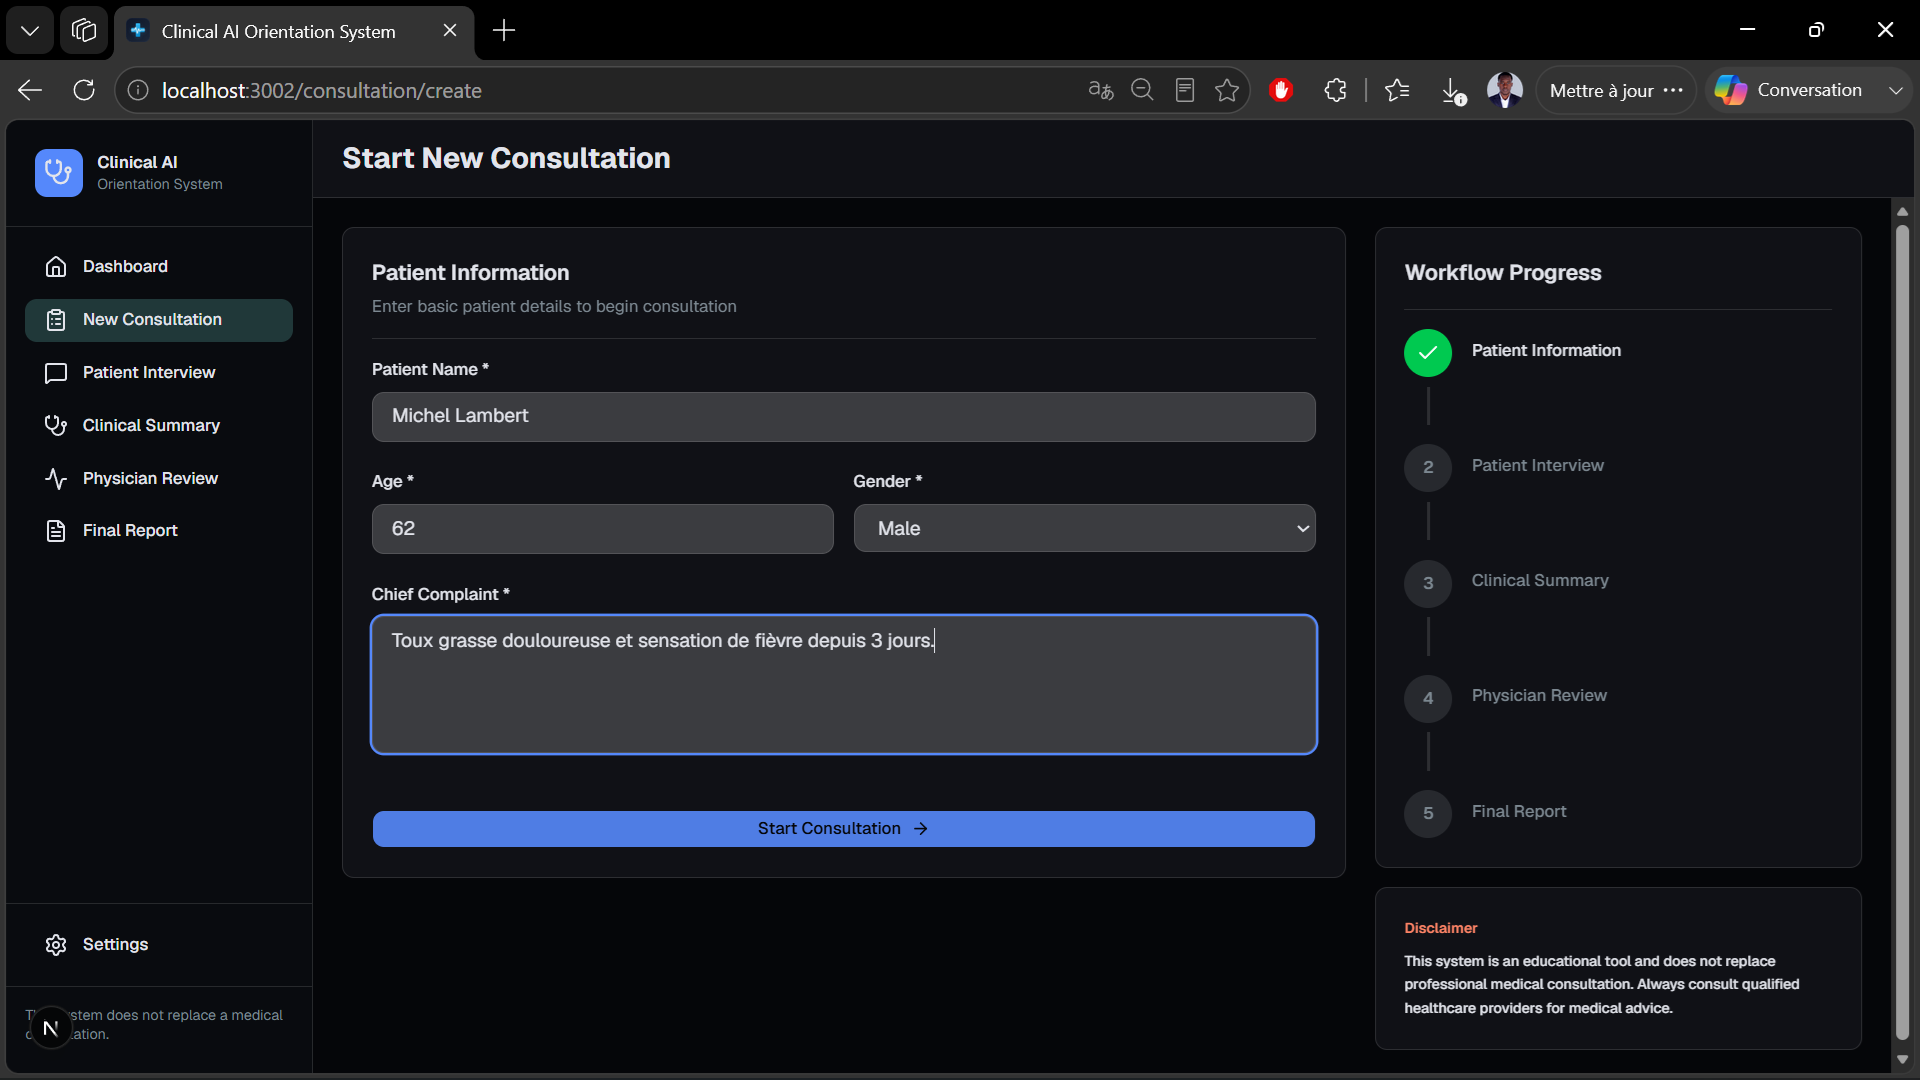
\includegraphics[width=0.75\textwidth]{dashboard.png}
\caption{Interface du tableau de bord clinique (Next.js).}
\label{fig:dashboard}
\end{figure}

\begin{figure}[H]
\centering
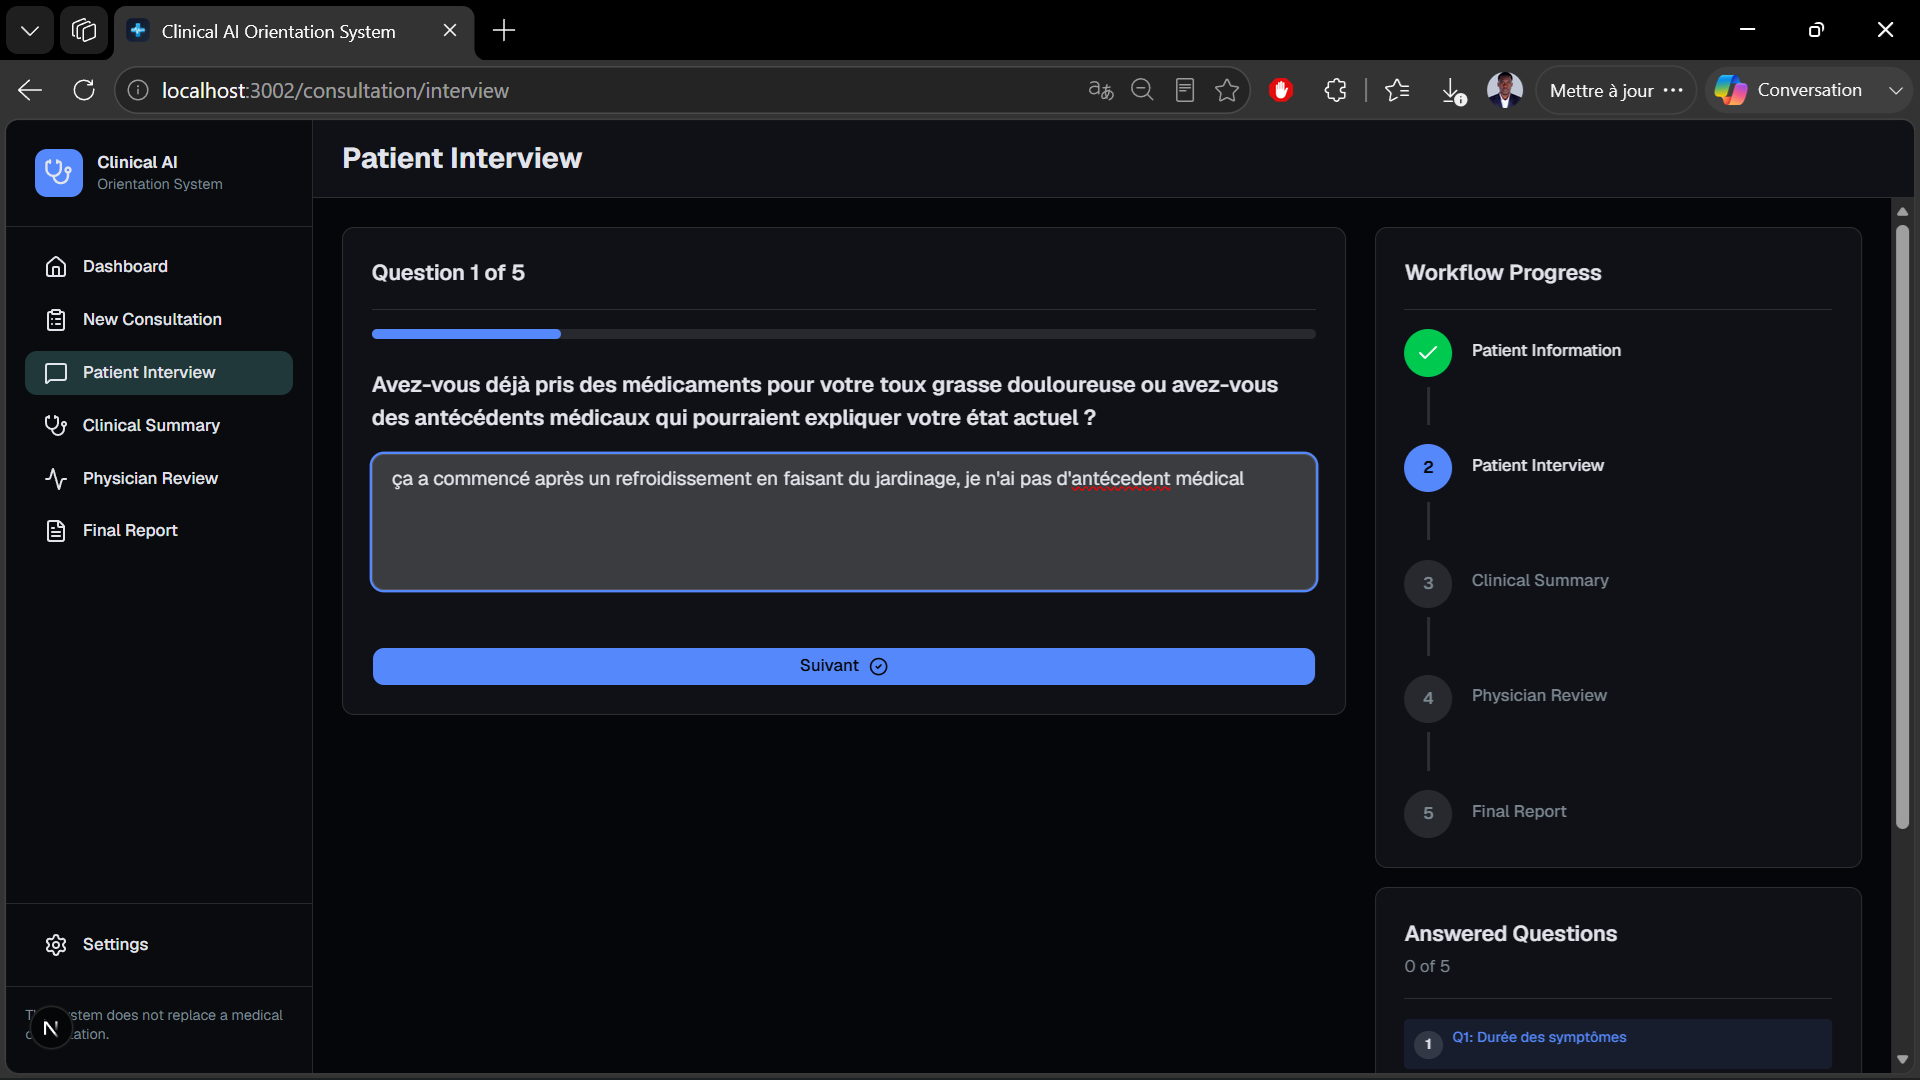
\includegraphics[width=0.75\textwidth]{new_consultation.png}
\caption{Formulaire d'admission pour une nouvelle orientation.}
\label{fig:new_consultation}
\end{figure}

\subsection{Entretien Interactif Conversationnel}
Dès l'admission validée, le patient accède à l'interface d'entretien interactif (Figure \ref{fig:question_flow}). Les questions s'enchaînent dynamiquement. Le volet de gauche affiche l'historique de la chronologie des échanges pour permettre au patient de suivre la progression.

\begin{figure}[H]
\centering
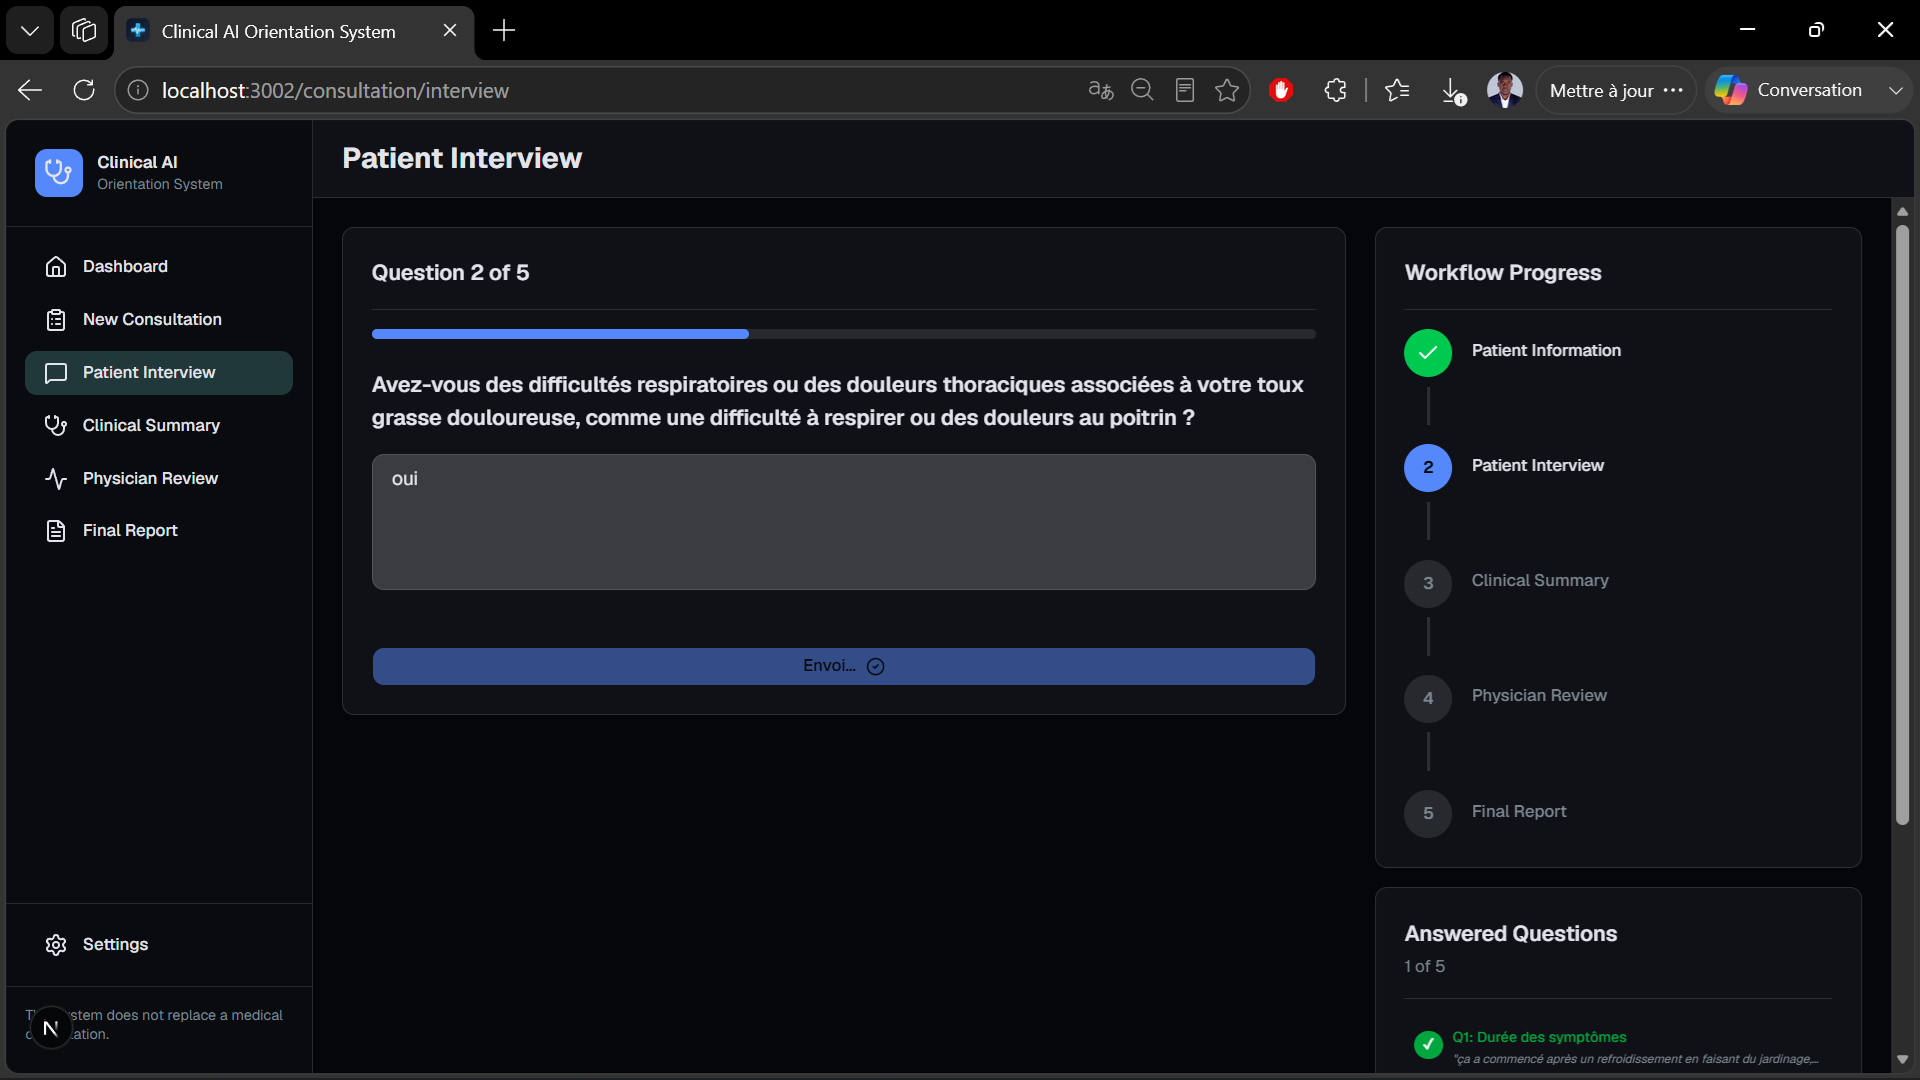
\includegraphics[width=0.75\textwidth]{question_1.png}
\caption{Première question générée dynamiquement par l'agent de diagnostic.}
\label{fig:question_flow}
\end{figure}

\subsection{Synthèse Clinique et Espace Médecin}
Une fois les 5 questions répondues, l'interface affiche la synthèse clinique intermédiaire, les recommandations provisoires et le niveau d'alerte calculé par l'outil de drapeaux rouges local (Figure \ref{fig:clinic_summary}). 
L'exécution du graphe se met en pause (HITL) et redirige vers l'espace de validation du médecin (Figure \ref{fig:physician_review}), où le médecin traitant saisit ses consignes et son plan de traitement.

\begin{figure}[H]
\centering
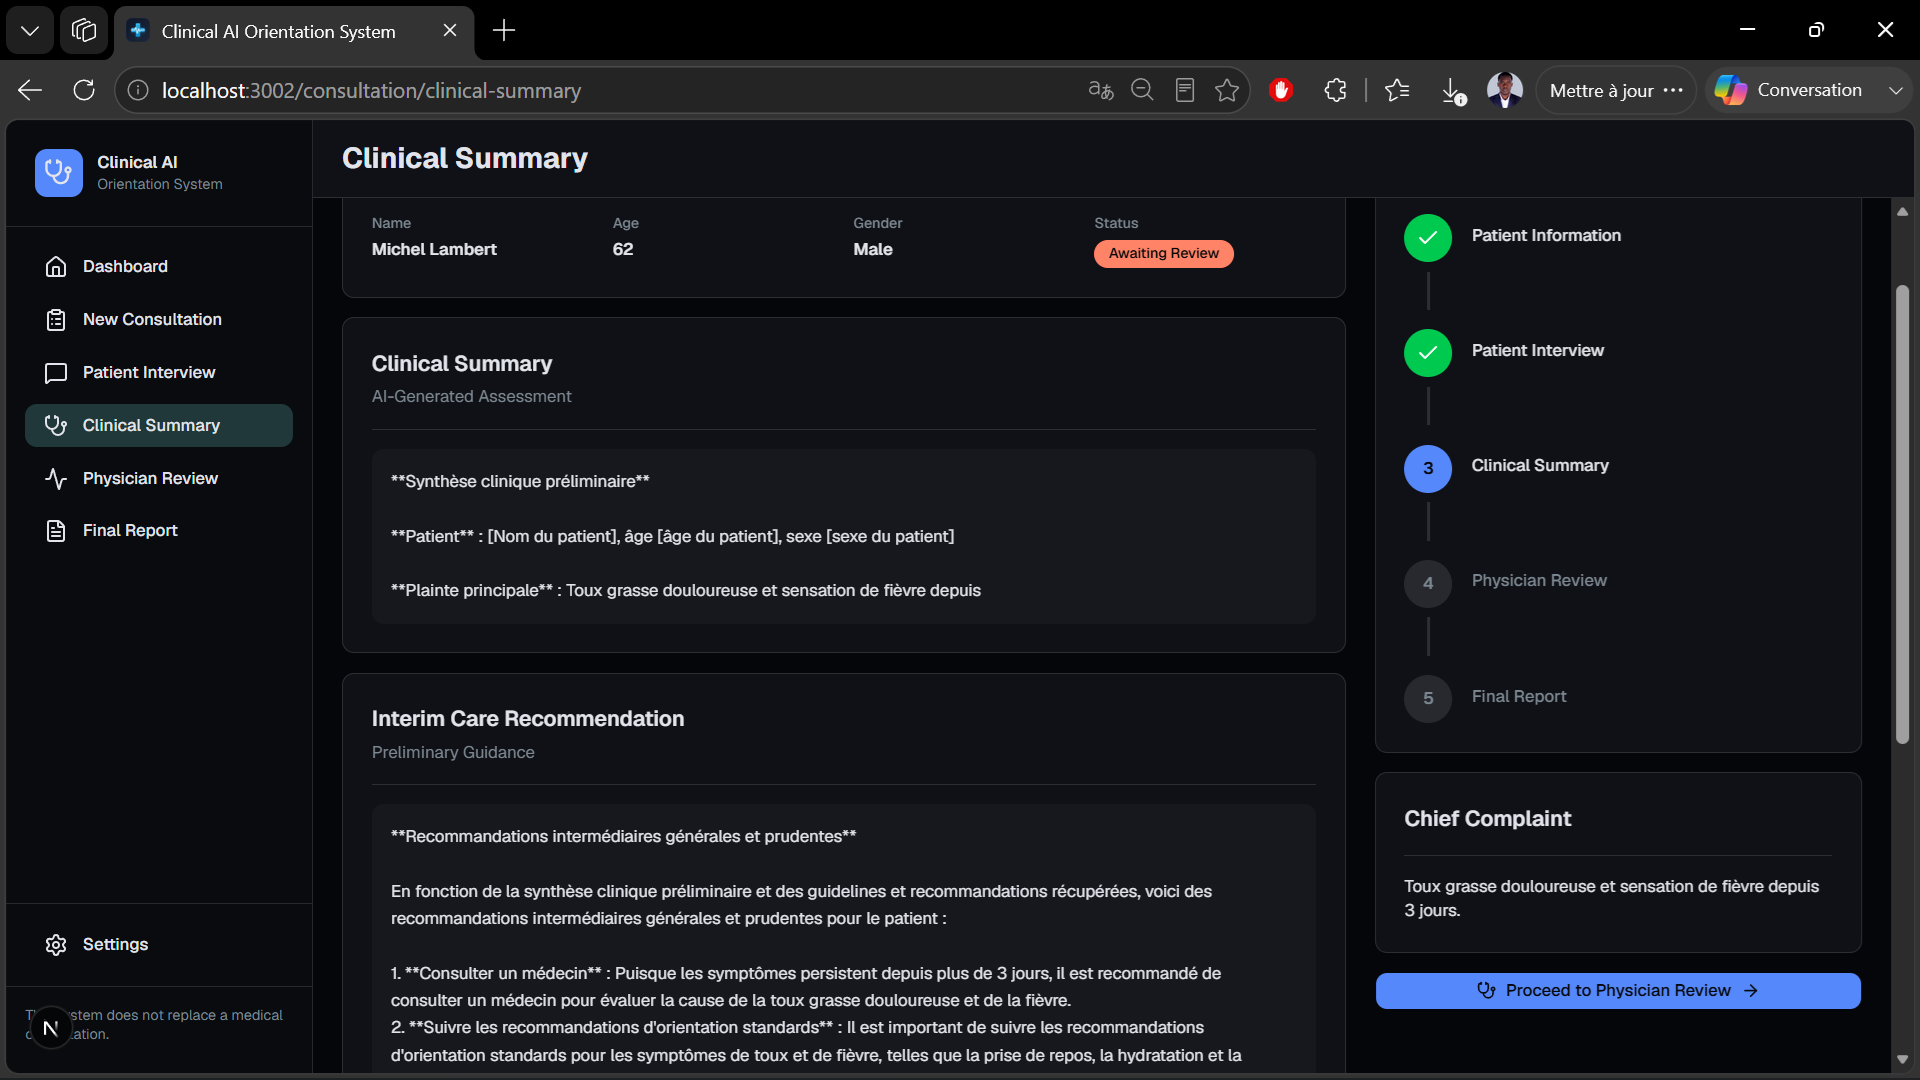
\includegraphics[width=0.75\textwidth]{clinic_summary.png}
\caption{Synthèse clinique préliminaire générée en attente d'avis médical.}
\label{fig:clinic_summary}
\end{figure}

\begin{figure}[H]
\centering
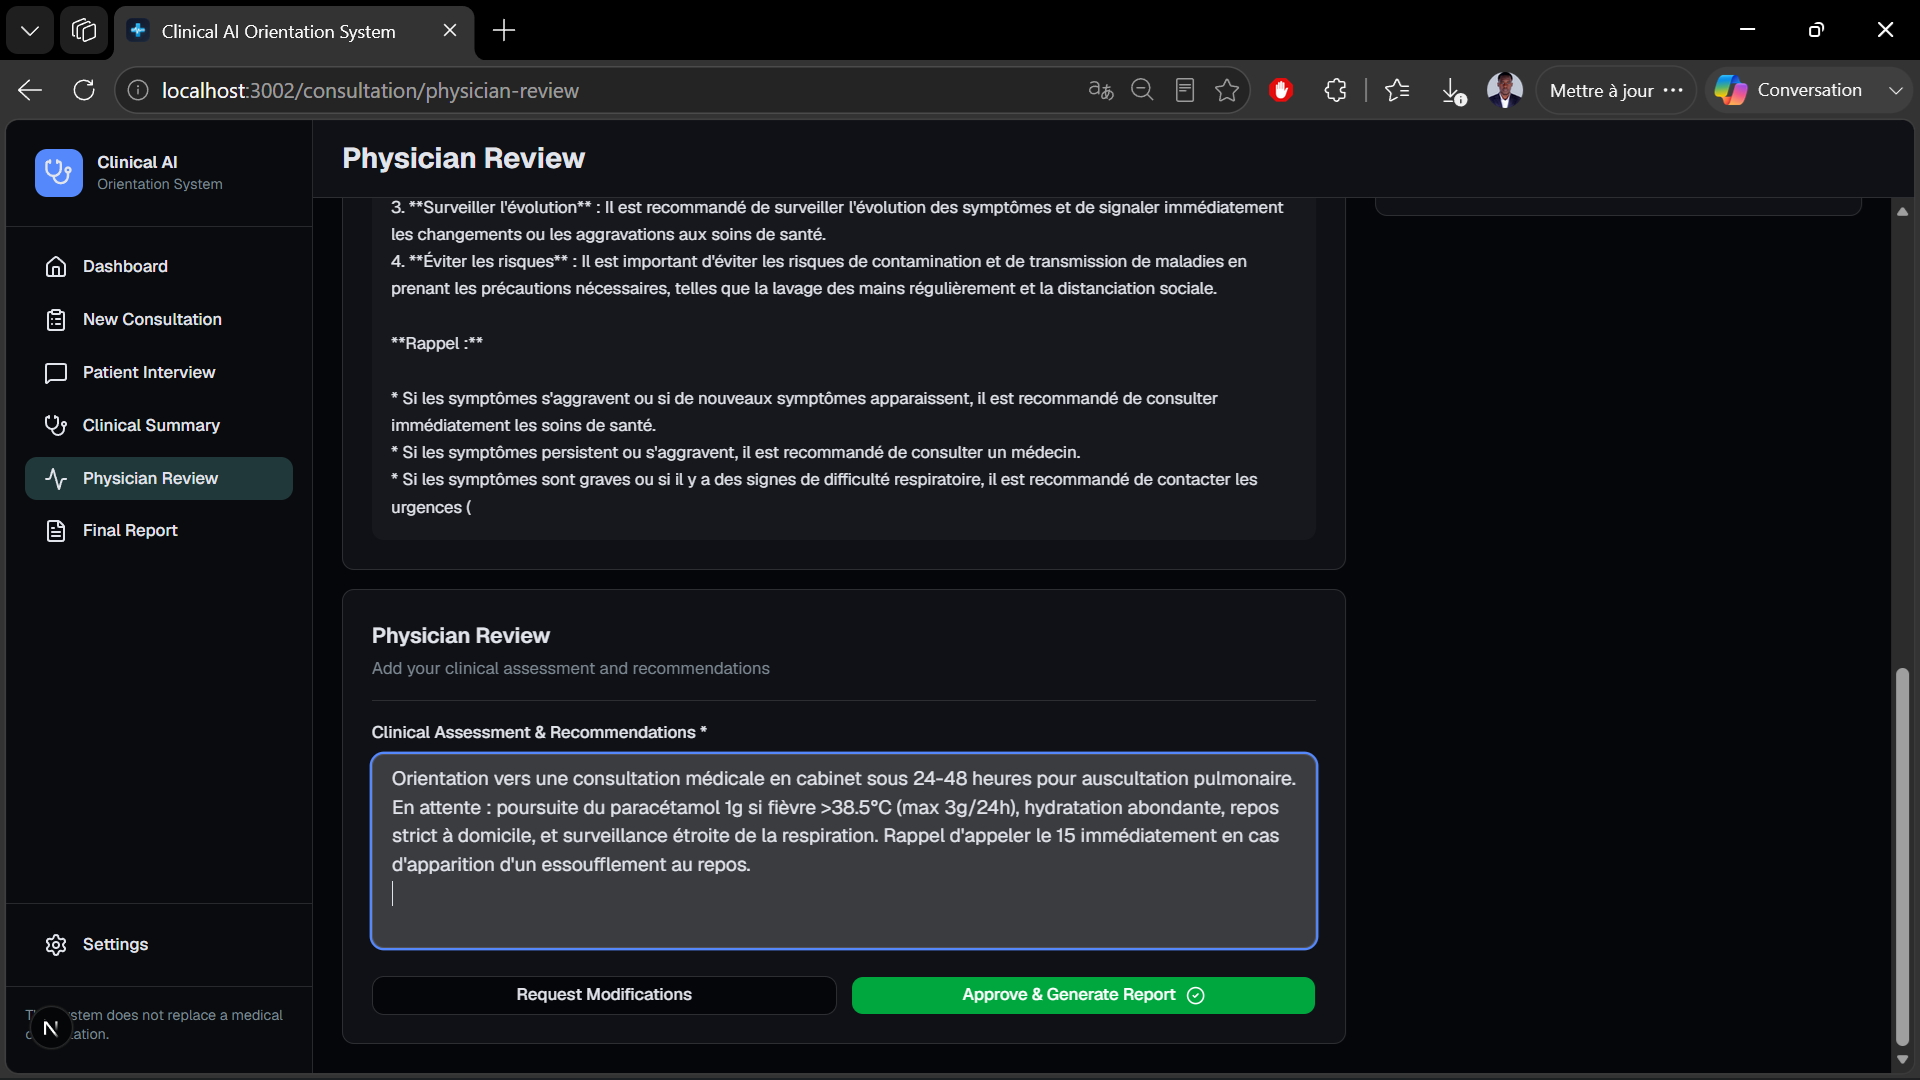
\includegraphics[width=0.75\textwidth]{physician_review.png}
\caption{Espace de saisie et de validation du médecin traitant.}
\label{fig:physician_review}
\end{figure}

\subsection{Rapport Final et Téléchargement}
Après validation par le médecin, le graphe est débloqué et le rapport final structuré s'affiche dans une console stylisée (Figure \ref{fig:final_report}). L'utilisateur ou le médecin peut immédiatement le copier ou le télécharger sous la forme d'un document PDF généré côté client (Figure \ref{fig:downloaded_report}).

\begin{figure}[H]
\centering
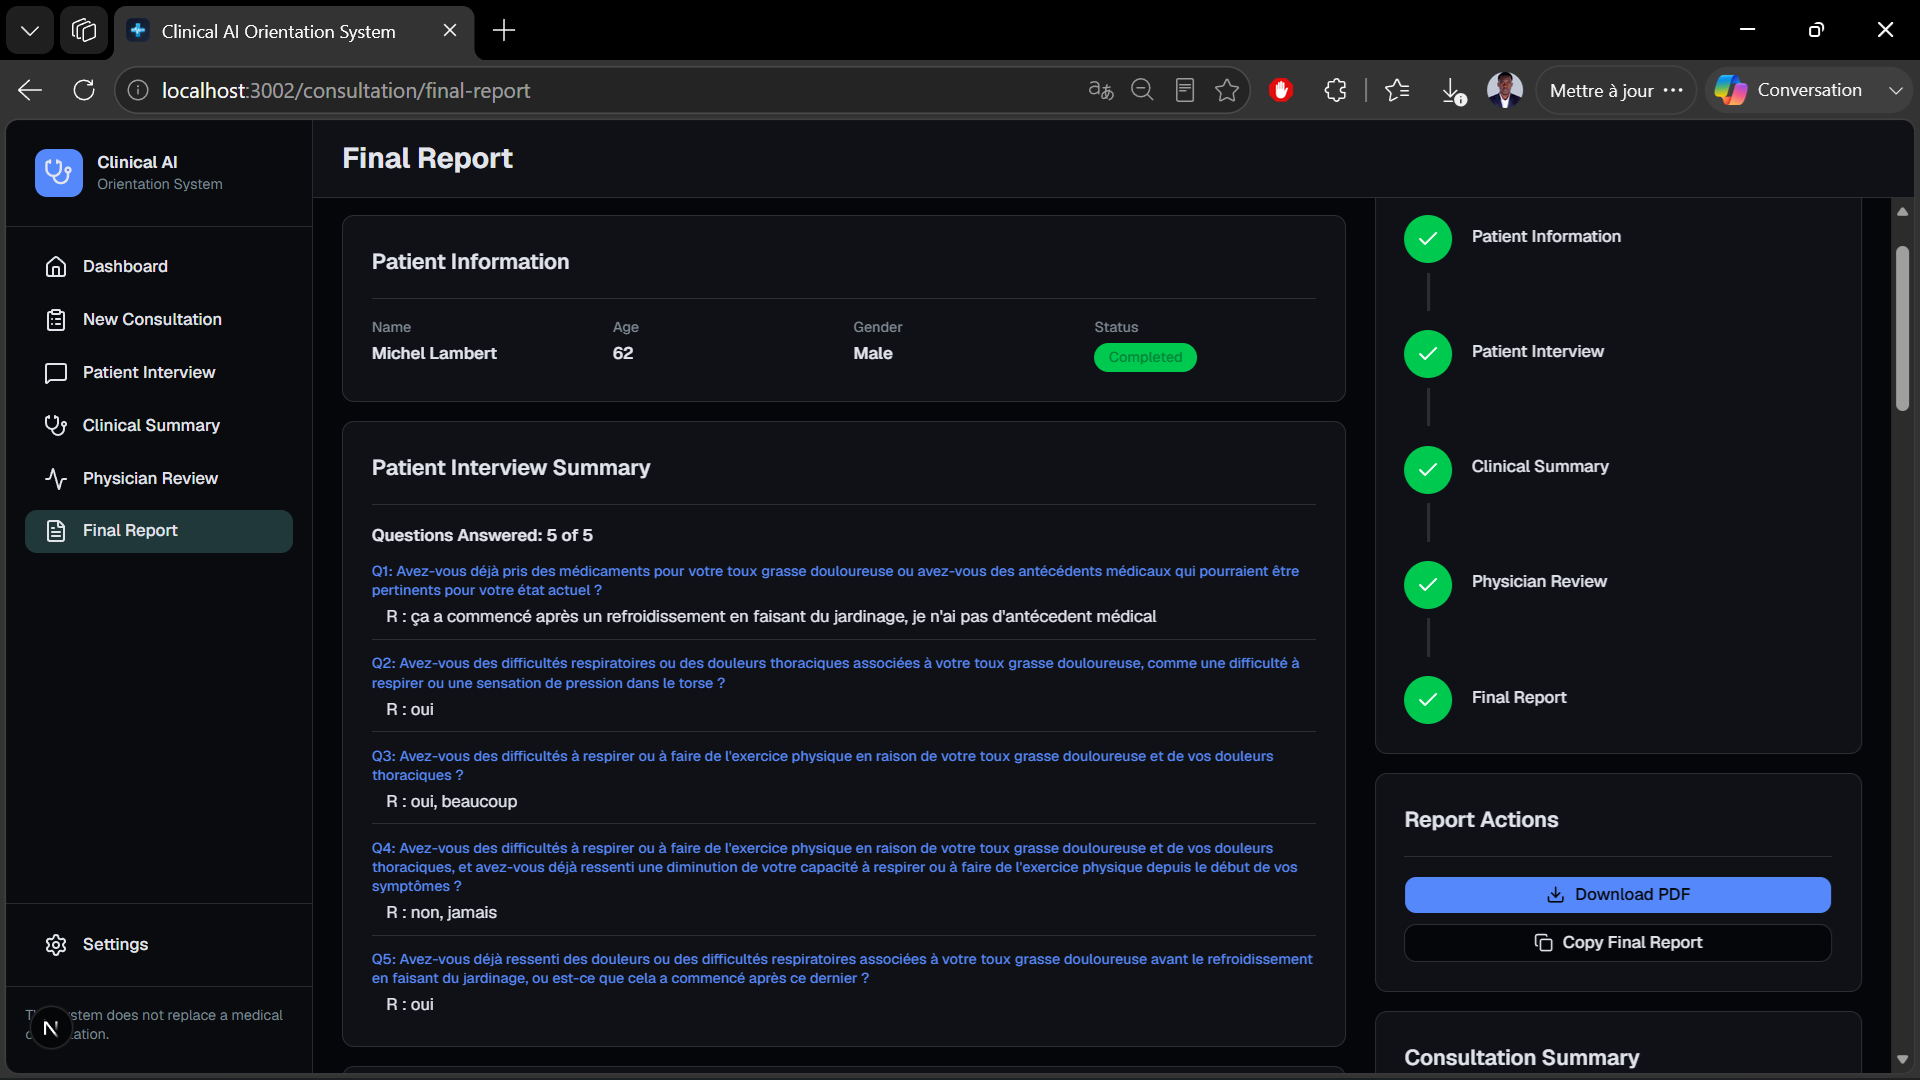
\includegraphics[width=0.75\textwidth]{final_report.png}
\caption{Rapport final structuré et consolidé disponible dans l'application.}
\label{fig:final_report}
\end{figure}

\begin{figure}[H]
\centering
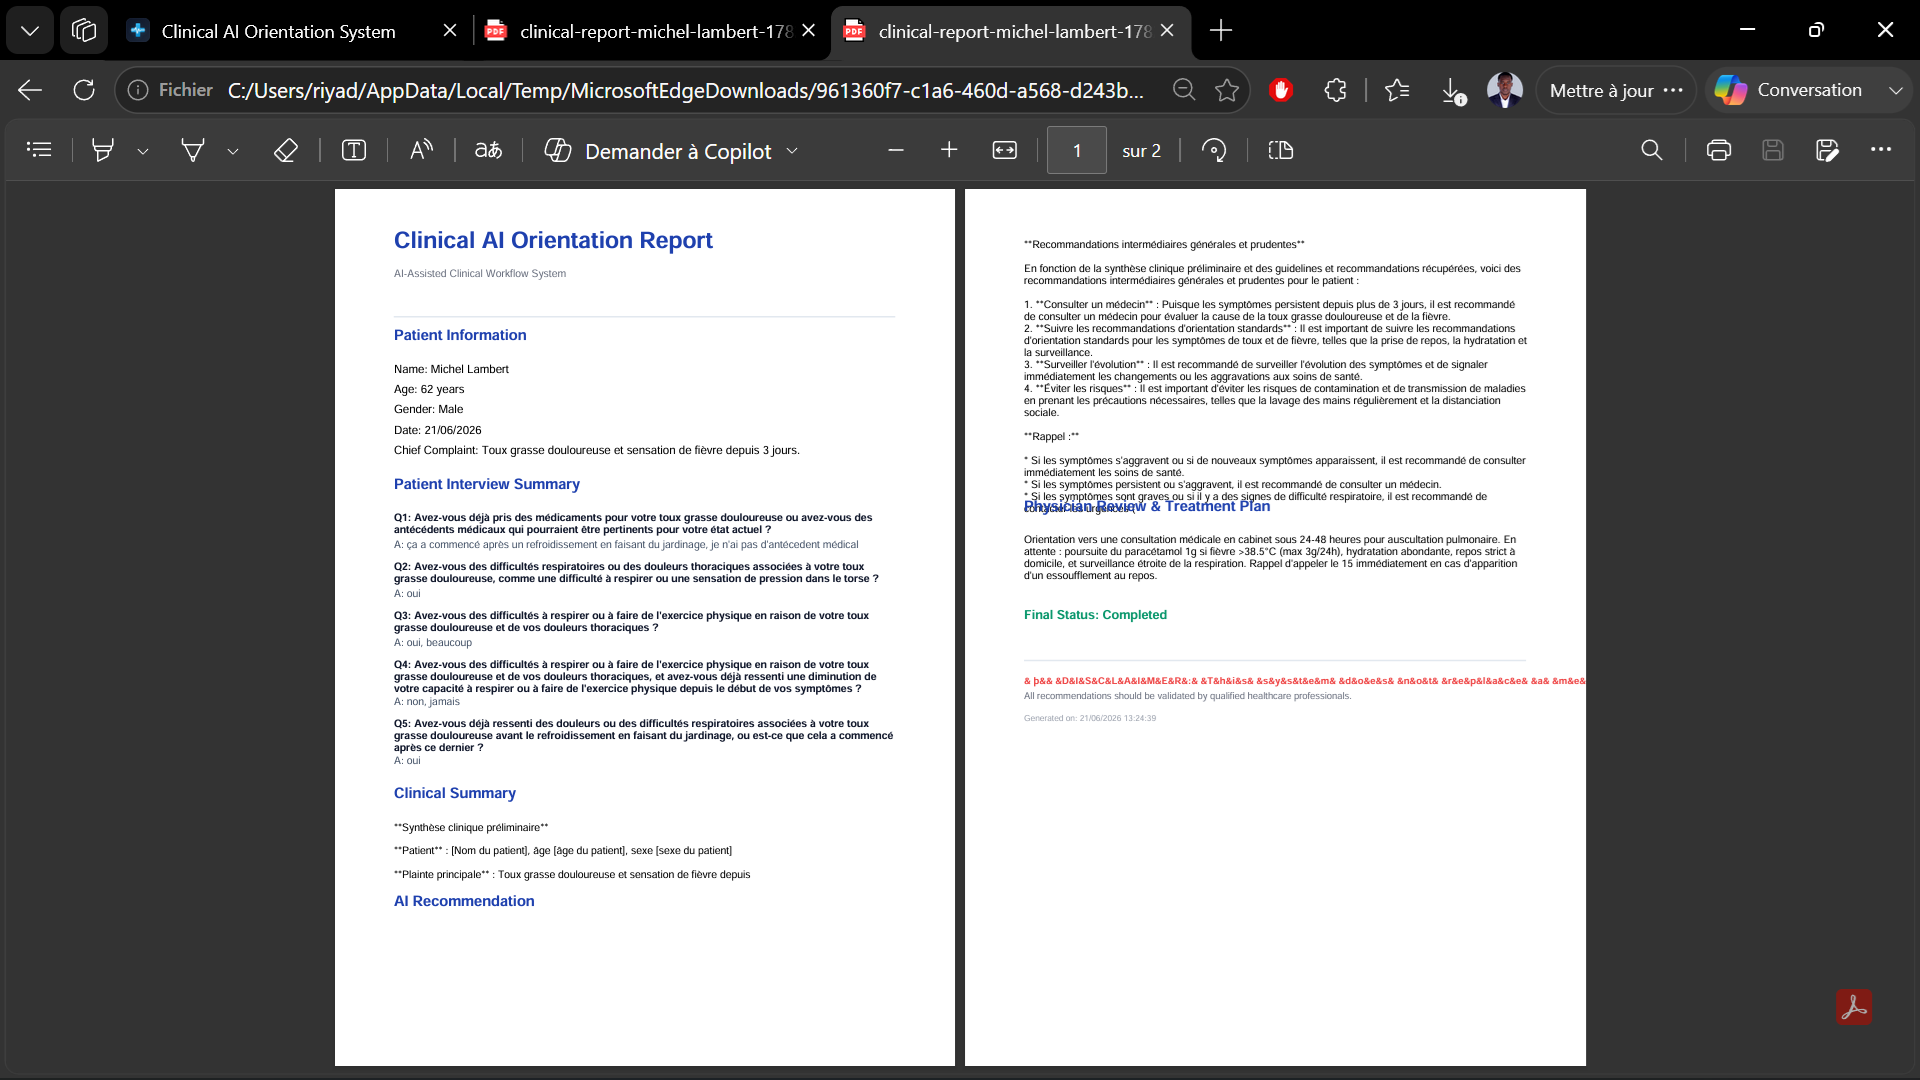
\includegraphics[width=0.55\textwidth]{downloaded_report.png}
\caption{Document PDF généré nativement via jsPDF côté client.}
\label{fig:downloaded_report}
\end{figure}

\chapter{Tests, Scénarios d'Orientation et Validation}
Ce chapitre présente les résultats d'orientation clinique obtenus sur deux cas d'usage réels, illustrant le fonctionnement autonome des agents conversationnels et la validation humaine systématique.

\section{Cas Clinique 1 : Syndrome Abdominal (Émilie Roux)}
Ce scénario met en avant l'adaptation dynamique de l'entretien clinique face à une suspicion de toxi-infection alimentaire ou gastro-entérite aiguë.

\subsection{Données d'Admission}
\begin{itemize}
    \item \textbf{Nom} : Émilie Roux | \textbf{Âge} : 24 ans | \textbf{Genre} : Féminin
    \item \textbf{Motif initial} : Nausées, vomissements et crampes abdominales depuis la nuit dernière.
\end{itemize}

\subsection{Entretien Clinique Dynamique}
L'agent de diagnostic interagit avec le patient sur 5 questions formulées en temps réel :
\begin{enumerate}
    \item \textbf{Q1} : Quelle est votre alimentation typique pendant les derniers jours, et avez-vous apporté des changements récents dans votre régime alimentaire ?
    \\ \textbf{R1} : \textit{Depuis deux jours, j'ai mangé plusieurs repas à l'extérieur, notamment un sandwich au poulet et une salade dans un restaurant. Je n'ai pas fait de changement particulier dans mon alimentation habituelle, mais certains aliments ne me semblaient pas très frais.}
    \item \textbf{Q2} : Avez-vous déjà pris des médicaments ou consommé des produits contenant des substances qui pourraient agir sur votre système digestif, tels que les antacides, les anti-inflammatoires non stéroïdiens (AINS) ou les diurétiques ?
    \\ \textbf{R2} : \textit{Oui, j'ai pris de l'ibuprofène hier pour un mal de tête, mais je ne prends pas habituellement d'autres médicaments et je n'ai pas utilisé d'antacides ou de diurétiques récemment.}
    \item \textbf{Q3} : Avez-vous ressenti des douleurs ou des ballonnements abdominaux, ou avez-vous eu des déjections anormales, notamment après avoir consommé le sandwich au poulet et la salade dans le restaurant ?
    \\ \textbf{R3} : \textit{Oui, quelques heures après avoir mangé le sandwich et la salade, j'ai commencé à ressentir des crampes abdominales et des ballonnements. J'ai également eu plusieurs épisodes de diarrhée depuis cette nuit.}
    \item \textbf{Q4} : Avez-vous déjà été exposée à un agent pathogène, tel qu'une bactérie, un virus ou un parasite, qui pourrait être à l'origine de vos symptômes actuels de nausées, vomissements et crampes abdominales ?
    \\ \textbf{R4} : \textit{Pas que je sache. Je n’ai pas été malade récemment et je n’ai pas eu de contact avec des personnes présentant des symptômes similaires. Je n’ai pas voyagé non plus et je ne pense pas avoir été exposée à une infection particulière.}
    \item \textbf{Q5} : Avez-vous déjà été enceinte ou avez-vous eu des problèmes de grossesse dans le passé, et avez-vous des antécédents familiaux de maladies digestives ou de problèmes de santé liés à la grossesse ?
    \\ \textbf{R5} : \textit{Non, je n’ai jamais été enceinte. Dans ma famille, il n’y a pas d’antécédents connus de maladies digestives ou de complications liées à la grossesse.}
\end{enumerate}

\subsection{Évaluation Clinique Intermédiaire et Avis du Médecin}
À la fin de l'entretien, le serveur MCP est consulté :
\begin{itemize}
    \item \textbf{Recherche RAG} : Association des symptômes gastro-intestinaux avec une suspicion de gastro-entérite aiguë ou intoxication alimentaire. Récupération des conseils d'hydratation orale.
    \item \textbf{Drapeaux Rouges} : Absence de signes de gravité. Statut de risque : \texttt{LOW}.
\end{itemize}
L'exécution est interrompue. Le médecin de garde examine le dossier et soumet le plan de traitement suivant :
\begin{quote}
    \textit{« After reviewing the case, the symptoms are most consistent with acute gastroenteritis likely of foodborne origin. Supportive treatment with hydration and rest. Avoid NSAIDs. »}
\end{quote}

\subsection{Rapport Final Structuré Généré}
\begin{lstlisting}[basicstyle=\ttfamily\tiny, frame=single, caption=Rapport final stocke en base pour Emilie Roux]
============================================================
          RAPPORT CLINIQUE D'ORIENTATION PRELIMINAIRE
============================================================
INFORMATIONS PATIENT
---------------------
Nom : Emilie Roux
Age : 24 ans | Genre : Feminin
Motif initial : Nausees, vomissements et crampes abdominales depuis la nuit derniere.

RESULTATS DE L'ORIENTATION
---------------------------
Synthese clinique :
Symptomes gastro-intestinaux aigus (vomissements, crampes, diarrhee) survenus quelques heures apres la consommation d'un repas suspect au restaurant (poulet). Evaluation: suspicion de gastro-enterite d'origine alimentaire. Pas de signe de gravite immediate detecte (Niveau de risque : LOW).

Recommandations temporaires :
1. Hydratation par petites gorgees regulieres.
2. Repos complet a domicile.
3. Eviter la prise d'ibuprofene (AINS pouvant aggraver l'irritation gastrique).

Avis et Traitement du medecin :
After reviewing the case, the symptoms are most consistent with acute gastroenteritis likely of foodborne origin. Supportive treatment with hydration and rest. Avoid NSAIDs.

------------------------------------------------------------
[!] AVERTISSEMENT : Ce systeme ne remplace pas une consultation medicale.
============================================================
\end{lstlisting}

\newpage
\section{Cas Clinique 2 : Infection Respiratoire (Michel Lambert)}
Ce scénario met en avant l'identification de signes de gravité modérés (difficulté respiratoire et douleurs thoraciques) nécessitant une auscultation clinique rapide.

\subsection{Données d'Admission}
\begin{itemize}
    \item \textbf{Nom} : Michel Lambert | \textbf{Âge} : 62 ans | \textbf{Genre} : Masculin
    \item \textbf{Motif initial} : Toux grasse douloureuse et sensation de fièvre depuis 3 jours.
\end{itemize}

\subsection{Entretien Clinique Dynamique}
L'agent conversationnel a orienté son questionnement sur la recherche de signes cardiorespiratoires :
\begin{enumerate}
    \item \textbf{Q1} : Avez-vous déjà pris des médicaments pour votre toux grasse douloureuse ou avez-vous des antécédents médicaux qui pourraient être pertinents pour votre état actuel ?
    \\ \textbf{R1} : \textit{Ça a commencé après un refroidissement en faisant du jardinage, je n'ai pas d'antécédent médical.}
    \item \textbf{Q2} : Avez-vous des difficultés respiratoires ou des douleurs thoraciques associées à votre toux grasse douloureuse, comme une difficulté à respirer ou une sensation de pression dans le torse ?
    \\ \textbf{R2} : \textit{Oui.}
    \item \textbf{Q3} : Avez-vous des difficultés à respirer ou à faire de l'exercice physique en raison de votre toux grasse douloureuse et de vos douleurs thoraciques ?
    \\ \textbf{R3} : \textit{Oui, beaucoup.}
    \item \textbf{Q4} : Avez-vous des difficultés à respirer ou à faire de l'exercice physique en raison de votre toux grasse douloureuse et de vos douleurs thoraciques, et avez-vous déjà ressenti une diminution de votre capacité à respirer ou à faire de l'exercice physique depuis le début de vos symptômes ?
    \\ \textbf{R4} : \textit{Non, jamais.}
    \item \textbf{Q5} : Avez-vous déjà ressenti des douleurs ou des difficultés respiratoires associées à votre toux grasse douloureuse avant le refroidissement en faisant du jardinage, ou est-ce que cela a commencé après ce dernier ?
    \\ \textbf{R5} : \textit{Oui.}
\end{enumerate}

\subsection{Évaluation Clinique Intermédiaire et Avis du Médecin}
L'analyse des réponses par les outils cliniques montre :
\begin{itemize}
    \item \textbf{Recherche RAG} : Association des symptômes respiratoires avec une bronchite aiguë ou pneumopathie débutante.
    \item \textbf{Drapeaux Rouges} : L'outil \texttt{red\_flag\_checker} identifie la présence de difficultés respiratoires et douleurs thoraciques. Le niveau de risque est évalué à \texttt{MODERATE}.
\end{itemize}
Le médecin traitant valide le dossier et ordonne une prise en charge rapide en cabinet :
\begin{quote}
    \textit{« Orientation vers une consultation médicale en cabinet sous 24-48 heures pour auscultation pulmonaire. En attente : poursuite du paracétamol 1g si fièvre >38.5°C (max 3g/24h), hydratation abondante, repos strict à domicile, et surveillance étroite de la respiration. Rappel d'appeler le 15 immédiatement en cas d'apparition d'un essoufflement au repos. »}
\end{quote}

\subsection{Rapport Final Structuré Généré}
Le listing suivant montre le rapport consolidé persistant pour Michel Lambert :

\begin{lstlisting}[basicstyle=\ttfamily\tiny, frame=single, caption=Rapport final stocke en base pour Michel Lambert]
============================================================
          RAPPORT CLINIQUE D'ORIENTATION PRELIMINAIRE
============================================================
INFORMATIONS PATIENT
---------------------
Nom : Michel Lambert
Age : 62 ans | Genre : Masculin
Motif initial : Toux grasse douloureuse et sensation de fievre depuis 3 jours.

RESULTATS DE L'ORIENTATION
---------------------------
Synthese clinique :
Symptomes respiratoires aigus (toux grasse douloureuse, sensation de fievre) accompagnes de difficultes respiratoires et douleurs thoraciques (Niveau de risque : MODERATE).

Recommandations temporaires :
1. Repos strict a domicile.
2. Hydratation abondante.
3. Prise de paracetamol si fievre >38.5C (max 3g/24h).
4. Eviter les efforts physiques.

Avis et Traitement du medecin :
Orientation vers une consultation medicale en cabinet sous 24-48 heures pour auscultation pulmonaire. En attente : poursuite du paracetamol 1g si fievre >38.5C (max 3g/24h), hydratation abondante, repos strict a domicile, et surveillance etroite de la respiration. Rappel d'appeler le 15 immediatement en cas d'apparition d'un essoufflement au repos.

------------------------------------------------------------
[!] AVERTISSEMENT : Ce systeme ne remplace pas une consultation medicale.
============================================================
\end{lstlisting}


\chapter{Limites Éthiques et Perspectives}
\section{Limites Actuelles}
\begin{itemize}
    \item \textbf{Dépendance aux API externes} : La qualité des questions dynamiques repose sur la disponibilité des clés OpenAI/OpenRouter.
    \item \textbf{Absence d'examens physiques} : L'orientation est purement déclarative et ne peut remplacer la palpation ou l'auscultation clinique.
\end{itemize}

\section{Perspectives}
\begin{itemize}
    \item \textbf{Intégration de Dossiers Médicaux Partagés (DMP)} : Permettre à l'agent de diagnostic de lire l'historique d'un patient pour affiner les questions.
    \item \textbf{Déploiement Cloud Sécurisé} : Migrer la base de données SQLite vers PostgreSQL dans un environnement certifié hébergeur de données de santé (HDS).
\end{itemize}

%===============================================================================
% CONCLUSION GENERALE
%===============================================================================
\newpage
\section*{Conclusion Générale}
\addcontentsline{toc}{section}{Conclusion Générale}

Ce projet de fin d'année a permis de concevoir et de réaliser une plateforme d'orientation clinique préliminaire multi-agents associant la flexibilité conversationnelle des LLM et la rigueur logicielle des graphes LangGraph. En intégrant des interruptions de sécurité (Red Flags locaux et validation humaine Physician-in-the-Loop) ainsi qu'un pipeline RAG dynamique (modèle MCP / Tavily), le système démontre qu'il est possible d'exploiter l'intelligence artificielle agentique dans un cadre médical simulé tout en maintenant un contrôle strict et éthique de l'information fournie au patient.

L'architecture moderne mise en place (FastAPI backend réactif et Next.js frontend) ainsi que les choix d'implémentation robustes (persistance SQLite résiliente et export de rapports PDF natifs stables) constituent une base technique solide. Ce prototype démontre l'intérêt concret des architectures de graphes d'agents supervisés pour modéliser des workflows complexes et interactifs dans les systèmes d'information de santé de demain.

%===============================================================================
% WEBOGRAPHIE / BIBLIOGRAPHIE
%===============================================================================
\newpage
\section*{Webographie}
\addcontentsline{toc}{section}{Webographie}

\subsection*{Frameworks et Orchestration}
\begin{itemize}
    \item LangGraph Orchestrator Documentation : \url{https://langchain-ai.github.io/langgraph/}
    \item FastAPI REST framework : \url{https://fastapi.tiangolo.com/}
    \item Next.js React Framework : \url{https://nextjs.org/docs}
\end{itemize}

\subsection*{Protocoles et Outils de Recherche}
\begin{itemize}
    \item Model Context Protocol (MCP) SDK : \url{https://modelcontextprotocol.io/}
    \item Tavily Search API documentation : \url{https://tavily.com/}
    \item SQLite database driver for Python : \url{https://docs.python.org/3/library/sqlite3.html}
    \item jsPDF documentation : \url{https://rawgit.com/MrRio/jsPDF/master/docs/index.html}
\end{itemize}

\subsection*{Dépôt de Code Source}
\begin{itemize}
    \item Dépôt GitHub officiel du projet : \url{https://github.com/riyadh03/IA_medical_assistant}
\end{itemize}

\end{document}
